\chapter{Supplementary material}
\label{supplementary-material}
\newpage
\begin{figure}[H]
	\centering
	\includegraphics[scale=0.7]{joint-hist-reg-tol.pdf}
	\caption{A comparison of the marginal ABC posterior (blue), sampled by the diagnostic ABC joint inversion, and the analytically defined posterior (red), sampled by MCMC, for a subset of the parameter space. This is the PDF which underlies the experiment in section \ref{SGE} and figures \ref{comparison-trunc}, \ref{grav-trunc} and \ref{tom-trunc}. The tolerance here is $\epsilon = \vec{1}\cdot0.1$. The black dashed lines marks the `true' parameter values from figures \ref{true-model-large-grav} and \ref{true-model-tom}. This ABC posterior can be compared to the ABC posterior for the same problem with $\epsilon = \vec{1}\cdot0.05$, figure \ref{pdf-half-tol} and $\epsilon = \vec{1}\cdot0.025$, figure \ref{pdf-quart-tol}. The parameters are numbered down column, starting with `1' in the top left corner (figure \ref{true-model-large-grav}).}
	\label{pdf-reg-tol}
\end{figure}

\begin{figure}[H]
	\centering
	\includegraphics[scale=0.7]{marginals-reg-tol.pdf}
	\caption{A comparison of Markov chain traces for the sampling of the ABC (blue) and analytically-defined (red) posteriors undertaken in section \ref{SGE}. The Markov chains are both of length 100,000. This figure is limited to a subset of 8 parameters out of the 120 total unknowns. The marginal histograms associated with each chain are also displayed. The black line marks the `true' parameter values from figures \ref{true-model-large-grav} and \ref{true-model-tom}. The parameters are numbered down column, starting with `1' in the top left corner (figure \ref{true-model-large-grav}).}
	\label{marginal-reg-tol}
\end{figure}

\begin{figure}[H]
	\centering
	\includegraphics[scale=0.65]{half-tol-joint-hist.pdf}
	\caption{A comparison of the marginal ABC posterior (blue), sampled by the diagnostic ABC joint inversion, and the analytically defined posterior (red), for a repetition of the experiment in section \ref{SGE} with a lower tolerance in the ABC likelihood approximation $p(\bm{S}(\bm{y})|\bm{S}(\bm{y^*},\bm{\theta}))$. The tolerance here is $\epsilon = \vec{1}\cdot0.05$, half the tolerance of the original experiment documented in section \ref{SGE}. The black dashed lines marks the `true' parameter values from figures \ref{true-model-large-grav} and \ref{true-model-tom}. This ABC posterior can be compared to the ABC posterior for the original experiment, figure \ref{pdf-half-tol} and an ABC posterior with $\epsilon = \vec{1}\cdot0.025$, figure \ref{pdf-quart-tol}. The sampling acceptance rate of the ABC posterior documented in this figure is 2.635\%, and the auto-correlation time ($\tau$) is 7892, figure \ref{comparison-quart-tol}.}
	\label{pdf-half-tol}
\end{figure}

\begin{figure}[H]
	\centering
	\includegraphics[scale=0.7]{quart-tol-hist.pdf}
	\caption{}
	\label{pdf-quart-tol}
\end{figure}

\begin{figure}[H]
	\centering
	\includegraphics[scale=0.8]{half-tol-comparison.pdf}
	\caption{}
	\label{comparison-half-tol}
\end{figure}

\begin{figure}[H]
	\centering
	\includegraphics[scale=0.8]{quart-tol-comparison.pdf}
	\caption{}
	\label{comparison-quart-tol}
\end{figure}

\begin{figure}[H]
	\centering
	\includegraphics[scale=1.1]{skew_updates.pdf}
	\caption{The skew Gaussian proposal distributions which can be used to positively or negatively bias the parameter update as an alternative to the truncated Gaussian distribution, figure \ref{updates}. The positively skewed distribution (a) is used when the parameter values are deemed too low. The negatively skewed distribution (b) is used when the parameter values are deemed too high. During application the distributions are centered on the current chain and $\omega = 250$.}
	\label{skew-updates}
\end{figure}

\begin{figure}[H]
	\centering
	\includegraphics[scale=0.8]{comparison-skew.pdf}
	\caption{Skew Gaussian scheme. The normalized misfit of the chain state during the initial phase (first 10,000 steps) for both datasets, $\Delta g$ and $\Delta t$, and for both methods, an analytically defined posterior sampled by MCMC and ABC-tomography. The `true model' and observed data is plotted in figure \ref{true-model-large-grav} and \ref{true-model-tom}. The increase in the rate of convergence to a low misfit model under ABC-tomography is a result of dynamically selecting, localizing and directly the update at each time step in the Markov chain. The details of the full chain run (100,000 time steps), are also displayed on the figure. $\tau$ is the integrated auto-correlation time. The mean marginal models from ABC-tomography using skew Gaussian updates is plotted in figure \ref{grav-skew} and \ref{tom-skew}.}
	\label{comparison-skew}
\end{figure}

\begin{figure}[H]
	\centering
	\includegraphics[scale=0.7]{abc_im-skew.pdf}
	\caption{Skew Gaussian scheme. The mean of the marginal ABC posterior, $p_{ABC}(\bm{\theta}|\bm{S}(\bm{y}))$, targeting the `true model' and observed data of figure \ref{true-model-large-grav}. The simulated data generated by this `solution', is plotted, blue, compared to the observed data, black. The misfit during the initial phase for this chain is plotted in figure \ref{comparison-skew}. The corresponding mean marginal $V_p$ model is plotted in figure \ref{tom-skew}.}
	\label{grav-skew}
\end{figure}

\begin{figure}[H]
	\centering
	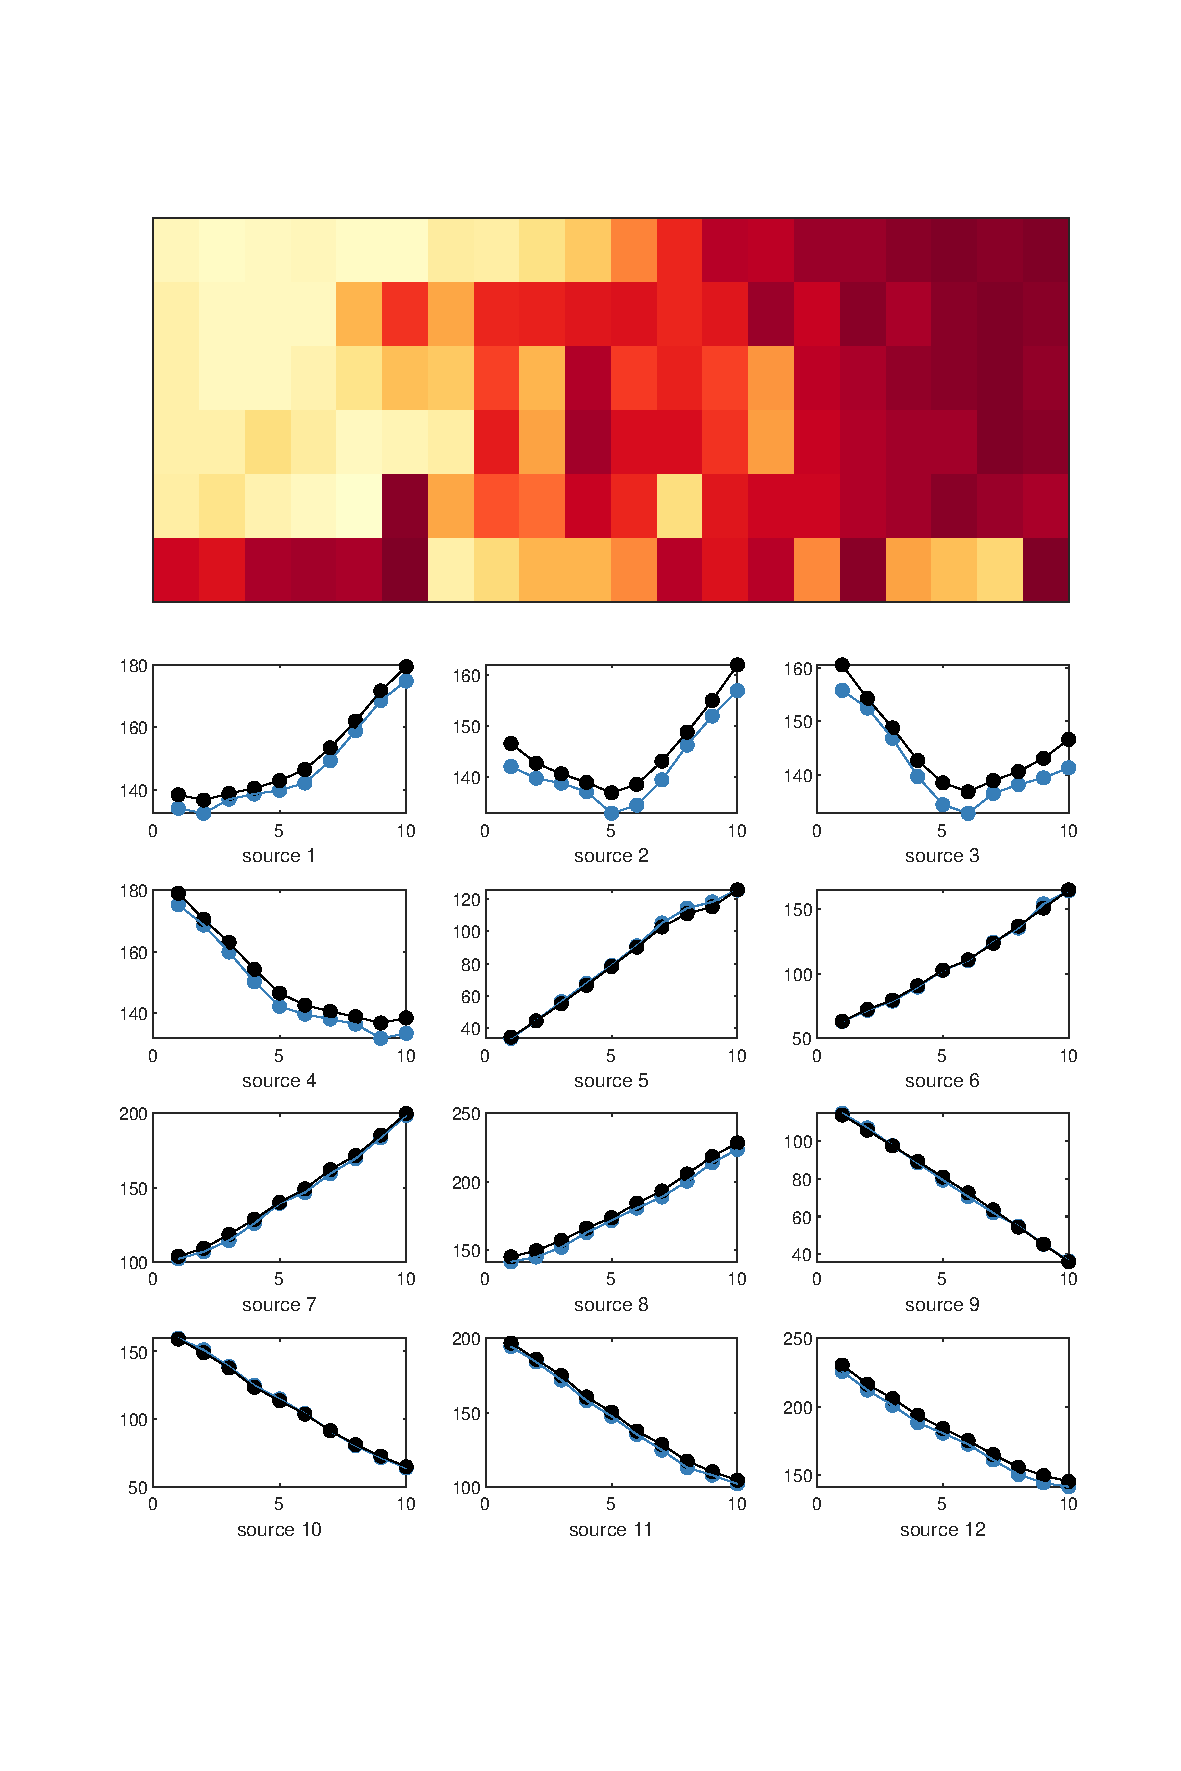
\includegraphics[scale=0.7]{abc-skew.pdf}
	\caption{Skew Gaussian scheme. The mean of the marginal ABC posterior, $p_{ABC}(\bm{\theta}|\bm{S}(\bm{y}))$, targeting the `true model' and observed data of figure \ref{true-model-tom}. The simulated data generated by this `solution', is plotted, blue, compared to the observed data, black. The misfit during the initial phase for this chain is plotted in figure \ref{comparison-skew}. The corresponding mean marginal $\rho$ model is plotted in figure \ref{grav-skew}.}
	\label{tom-skew}
\end{figure}
